\subsection{Кинематика точки}

\subsubsection*{1.12*}
Параметризуем движение точки некоторым $\varphi(t)$:
\begin{equation}
\label{strsin}
    \left\{\begin{aligned}
        x =  a \cos \varphi\\ 
        y =  b \sin \varphi
    \end{aligned}\right. 
    \hspace{0.25cm} \Rightarrow \hspace{0.25cm} 
    \left\{\begin{aligned}
        \dot{x} &= - a \dot{\varphi} \sin \varphi \\
        \dot{y} &= b \dot{\varphi} \cos \varphi
    \end{aligned}\right.
    \hspace{0.25cm} \Rightarrow \hspace{0.25cm} 
    \left\{\begin{aligned}
        \ddot{x} &= -a \dot{\varphi}^2 \cos \varphi - a \ddot{\varphi} \sin \varphi = 0 \\
        \ddot{y} &= -b \dot{\varphi}^2 \sin \varphi + b \ddot{\varphi} \cos \varphi 
    \end{aligned}\right.
    \hspace{0.25cm} \Rightarrow \hspace{0.25cm} 
    \dot{\varphi}^2 + \ddot{\varphi} \tg \varphi = 0.
\end{equation}
Решением этого уравнения является
$$
    \varphi(t) = \arccos (c_1 + c_2 t).
$$
С учётом начальных условий получим ($x(0)=0$, $\dot{x} = $), что
$$
    \dot{\varphi} 
    c_1 = 0,\hspace{0.5cm} c_2 = \frac{v_0}{a},
    \hspace{0.5cm} \Rightarrow \hspace{0.5cm} 
    \varphi(t) = \arccos (v_0 t / a).
$$
Немного упростим выражения для $\dot{\varphi}$ и $\ddot{\varphi}$:
$$
    \dot{\varphi} = -\frac{v_0}{a \sin \varphi}, \hspace{0.25cm} 
    \ddot{\varphi} = - \frac{\dot{\varphi}^2}{\tg \varphi},
$$
теперь найдём $\ddot{y} (\sin \varphi)$:
$$
    \ddot{y} = - b \dot{f} \sin \varphi + v \ddot{\varphi} \cos \varphi =
    -b \frac{v_0^2}{a^2 \sin^2 \varphi} \sin \varphi - b \left(\frac{v_0}{a} \right)^2 \frac{\cos \varphi}{\sin^2 \varphi \tg \varphi} = 
    - \frac{b}{a^2} v_0^2 \left(\frac{1}{\sin \varphi} + \frac{\cos^2 \varphi}{\sin^3 \varphi} \right) = -\frac{b}{a^2} v_0^2 \frac{1}{\sin^3 \varphi}.
$$ 
Подставив $y = b \sin \varphi$, найдём
$$
    \ddot{y}\left(y = \frac{b}{2} \right) = -\frac{8b}{a^2} v_0^2. 
$$

\subsubsection*{1.19}

Знаем, что в полярных координатах
\begin{equation}
\label{1_2}
    \left\{\begin{aligned}
        r &= \frac{p}{1 + e \cos \varphi}  \\
        r^2 \dot{\varphi} &= c = \const
    \end{aligned}\right.
    \hspace{0.5cm} 
    \text{в полярных координатах}
    \hspace{0.5cm} 
    \left\{\begin{aligned}
        x &= r \cos \varphi \\
        y &= r \sin \varphi
    \end{aligned}\right.
    .    
\end{equation}
Вспомним, что
\begin{align*}
    w_r = \ddot{r} - r \dot{\varphi}^2, \hspace{0.5cm} 
    w_\varphi = \frac{d}{dt} \left(r^2 \dot{\varphi}\right).
\end{align*}
Найдём $\ddot{r}$:
$$
    r + er \cos \varphi = p
    \hspace{0.25cm} \overset{d / d t}{\Rightarrow} \hspace{0.25cm} 
    \dot{r} + e \dot{r} \cos \varphi - e r \dot{\varphi} \sin \varphi = 0
    \hspace{0.25cm} \overset{d / d t}{\Rightarrow} \hspace{0.25cm} 
    \ddot{r} (1 + e \cos \varphi) - e \dot{r} \sin \varphi \left(\dot{\varphi} - \frac{c}{r^2} \right) -\frac{ec}{r} \frac{c}{r^2} \cos \varphi = 0
$$
Выразим и подставим $\dot{\varphi}$ и получим
$$
    \dot{\varphi} = \frac{c}{r^2},
    \hspace{0.5cm} \Rightarrow \hspace{0.5cm} 
    \ddot{r} = \frac{c^2}{r^2 p} \left(\frac{p}{r} -1\right),
    \hspace{0.5cm} \Rightarrow \hspace{0.5cm} 
    \boxed{
    w_r = -\frac{c^2}{pr^2} , \hspace{0.5cm} 
    w_\varphi = 0.}
$$

\subsubsection*{1.37(в)}

Найдём скорость точки и проекции её ускорения на касательные к координатным линиям для координат параболического цилиндра $\sigma, \tau, z$. Для начала найдём координатные векторы и метрический тензор:
$$
    \vc{r} = \begin{pmatrix}
        x \\ y \\ z
    \end{pmatrix} = \begin{pmatrix}
        \sigma \tau \\ \frac{1}{2} (\tau^2 - \sigma^2) \\ z
    \end{pmatrix}
    \hspace{0.5cm} \Rightarrow \hspace{0.5cm} 
        \vc{g}_\sigma = \begin{pmatrix}
        \tau \\ - \sigma \\ 0 
    \end{pmatrix},
    \vc{g}_\tau = \begin{pmatrix}
        \sigma \\ \tau \\ 0
    \end{pmatrix},
    \vc{g}_z = \begin{pmatrix}
        0 \\ 0 \\ 1
    \end{pmatrix}, \hspace{0.5cm} 
    g_{ij} = \begin{pmatrix}
        \tau^2 + \sigma^2 & 0 & \\
        0 & \tau^2 + \sigma^2 & 0 \\
        0 & 0 & 1
    \end{pmatrix}.
$$
Тогда
$$
    v^2 = \dot{\sigma}^2 (\tau^2 + \sigma^2) + \dot{\tau}^2 (\tau^2 + \sigma^2) + \dot{z}^2,
    \hspace{0.5cm} 
    v =  \sqrt{(\dot{\tau}^2 + \dot{\sigma}^2)(\tau^2 + \sigma^2) + \dot{z}^2}
$$
Для $i$-ой ковариантной координаты ускорения верно, что
\begin{equation}
    w_i = \frac{d}{dt} \frac{\partial (v^2/2)}{\partial \dot{q}^i} - \frac{\partial (v^2/2)}{\partial q^i}.
\end{equation}
С учётом коэффициенты Ламе ($H_\tau = H_\sigma=\sqrt{\sigma^2+\tau^2}, H_z = 1$), найдём проекции
\begin{align*}
    w_\tau &= \frac{1}{\sqrt{\sigma^2+\tau^2}} \left(
        \ddot{\tau} (\tau^2 + \sigma^2) + \dot{\tau}^2 \tau  + 2 \dot{\sigma} \dot{\tau} \sigma - \tau \dot{\sigma}^2
    \right); \\
    w_\sigma &= \frac{1}{\sqrt{\sigma^2+\tau^2}} \left(
        \ddot{\sigma} (\tau^2 + \sigma^2) + \dot{\sigma}^2 \sigma  + 2 \dot{\tau} \dot{\sigma} \tau - \sigma \dot{\tau}^2\right); \\
    w_z &= \ddot{z}.
\end{align*}


\subsubsection*{1.45}
Выразим орты сопровождающий трехгранника $(\dot{\tau}, \vc{n}, \vc{b})$ через $\vc{v}$ и $\vc{w}$, с учётом $w \times \vc{v} \neq 0$, $\vc{t} \cdot \vc{v} > 0$.
Так как $\vc{v} \nparallel \vc{w}$, то
$$
    \vc{b} = \frac{\vc{v} \times \vc{w}}{|\vc{v} \times \vc{w}|}.
$$
Выразим $\vc{\tau}$.
$$
    \vc{\tau} = \frac{d \vc{r}}{d s}, \hspace{0.5cm} 
    \vc{v} = \frac{d \vc{r}}{d t} = \frac{ds}{dt} \frac{d \vc{r}}{ds} = v \dot{\tau},
    \hspace{0.5cm} \Rightarrow \hspace{0.5cm} 
    \vc{\tau} = \frac{\vc{v}}{v}.
$$
И найдём $\vc{n} = [\vc{b} \times \vc{\tau}]$, раскрывая двойное векторное произведение (формула Лагранжа), получим
$$
    \vc{n} = \left[\frac{\vc{v}}{v} \times \frac{\vc{v} \times \vc{w}}{|\vc{v} \times \vc{w}|}\right]=
    \frac{\left(\vc{w} \cdot \vc{v}\right)\vc{v} - v^2 \vc{w}}{v |\vc{v} \times \vc{w}|} .
$$

\subsubsection*{Т6.}

Рассмотрим движение точки в цилиндрических координатах:
$$
    \vc{r} = \begin{pmatrix}
        x \\ y \\ z  
    \end{pmatrix} = \begin{pmatrix}
        r \cos \varphi \\ r \sin \varphi \\ z
    \end{pmatrix}
    \hspace{0.5cm} \Rightarrow \hspace{0.5cm} 
    \vc{J} = \begin{pmatrix}
        \cos \varphi & - r \sin \varphi & 0 \\
        \sin \varphi & r \cos \varphi & 0 \\
        0 & 0 & 1
    \end{pmatrix}, \hspace{0.5cm} 
    g_{ij} = \diag(1, r^2, 1)
$$

\begin{wrapfigure}{r}{0.4\textwidth}
  \begin{center}
        \vspace{-5 mm}
        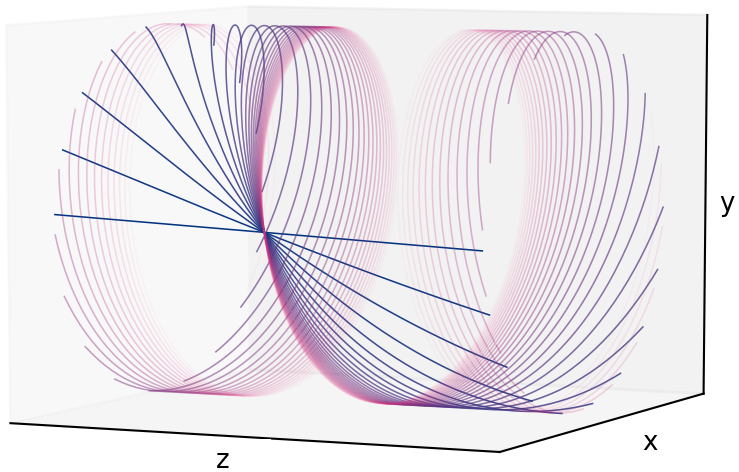
\includegraphics[width=0.9\linewidth]{img/T6_v2.png}
  \end{center}
    \caption{Возможные геодезические цилиндра.}
    \label{fig:cilindre}
\end{wrapfigure}

Для начала выразим ковариантные координаты ускорений:
$$
    w_i = \frac{d}{dt} \frac{\partial (v^2/2)}{\partial q\delta^i} - \frac{\partial (v^2/2)}{\partial q^i} 
    \hspace{0.5cm} \Rightarrow \hspace{0.5cm} 
    \left[\begin{aligned}
        w_r &= \ddot{r} - r \dot{f}^2 \\
        w_\varphi &= \frac{d}{dt} (r^2 \dot{\varphi}) \\
        w_z &= \ddot{z}.
    \end{aligned}\right.
$$
По условию хотим, чтобы $w_\varphi = w_z = 0, r=\const$. Проинтегрировав дважды по времени получим систему уравнений
$$
    \left\{\begin{aligned}
        \varphi &=  c_1 t + c_2;\\
        z &= c_3 t + c_4,
    \end{aligned}\right.
$$
Где $c_1, c_2, c_3, c_4$ --некоторые константы. Построим полученные траектории положив $c_2 = c_4 = 0$ и отмасштабировав к $c_1 = 1$ (см. рис. \eqref{fig:cilindre}).

% \newpage

\subsubsection*{Т7.}
Найдём $\partial v_k / \partial v_j$, при $v_k = v_k(q^i, v^i)$. Далее будем пользоваться тем, что $g_{ig} = g_{ig}(q^i)$.
$$
    v_k(q^i, v^i) = g_{ki} v^i 
    \hspace{0.5cm} \Rightarrow \hspace{0.5cm} 
    \frac{\partial v_k}{\partial v^j} = g_{ki} \frac{\partial v^i}{\partial v^j} = g_{ki} \delta^i_j = g_{kj}.
$$
Теперь найдём $\partial v_k / \partial q^j$, при $v_k = v_k(q^i, v^i)$. 
$$
    \frac{\partial v_k(q^i, v^i)}{\partial q^j} = v^i \left(
        \frac{\partial  g_{ki}}{\partial q^j} 
    \right) = v^i \left(
        \left(\frac{\partial \vc{g}_k}{\partial q^j}, \, \vc{g}_i \right) +
        \left(\frac{\partial \vc{g}_i}{\partial q^j}, \, \vc{g}_k\right)
    \right) = v^i\left(\Gamma_{ijk} + \Gamma_{kji}\right).
$$
Теперь найдём $\partial v_k / \partial q^j$, при $v_k = v_k(q^i, v_i)$. Но тут так как функция выражается через саму себя, то при частном дифференцировании, $v_k = \const$, тогда $\partial v_k(q^i, v_i) / \partial q^j = 0$.



\subsubsection*{Т8.*}
Найдём $v_i \dot{v}^i - v^i \dot{v}_i$. Перейдём к контравариантным координатам:
$$
    v_i \dot{v}^i - v^i \dot{v}_i = g_{ij} v^i v^j - v^i \frac{d}{dt} \left(
             g_{ij} v^j
        \right) =    g_{ij} v^j \dot{v}^i  - v^i v^j \dot{g}_{ij} - g_{ij} v^i \dot{v}^j
$$
В силу симметричности метрического тензора $g_{ij}=g_{ji}$, получим, что
$$
    v_i \dot{v}^i - v^i \dot{v}_i =  - v^i v^j \dot{g}_{ij}.
$$
Подставил для параболических и полярных координат, сходится.

